\documentclass[12pt]{article}

\usepackage{amsmath}
\usepackage{amssymb}
\usepackage{amsthm}
\usepackage{enumitem}
\usepackage{graphicx}
\usepackage{float}

\renewcommand{\arraystretch}{1.5} % Increases row spacing by a factor of 1.5

\title{MATH 307-101
Applied Linear Algebra}
\author{MacKenzie Richards, Ankkit Prakash, \\ Somesh Joshi, Cai Lewendon}
\date{2024 Winter Term 1 (Sep–Dec 2024)}
\begin{document}
\maketitle
\section{Approximating Eigenvalues with the QR Algorithm}
\subsection{Prove $A_1$ is similar to A}
\begin{proof}
    A is a square matrix. Let, $A = QR$ be the QR factorization of A. \\
    Q is a square matrix, and its columns form an orthonormal basis by construction. \\
    Therefore, $Q^{-1} = Q^T$ and $Q^{T}Q = QQ^T = I$, i.e, Q is invertible\\
    $A_1 = RQ$.\\ 
    A matrix $A$ is similar to another matrix $B$ if there exists an invertible matrix $P$ such that:
    $$A = PBP^{-1}$$
    For $B = A_1$ and $P = Q$ \\
    $$A = QR = QR(QQ^{-1}) = Q(RQ)Q^{-1} = QA_1Q^{-1}$$ \\
    Therefore, $A_1$ is similar to $A$. \\ 
    Now, to prove $A_1$ and $A$ have the same eigenvectors. \\
    A matrix has an eigenvalue $\lambda$ and corresponding eigenvector $v$ if \\
    $$Av = \lambda v$$
    Since $A = QA_1Q^{-1} = QA_1Q^{T}$
    $$QA_1Q^{T} v = \lambda v$$
    Left multiply both sides by $Q^T$
    $$ (Q^{T}Q) A_1 (Q^{T}v) = Q^{T} \lambda v = \lambda (Q^{T}v)$$ \\
    Set $u = Q^{T} v$. We get, \\
    $$ A_1 u = \lambda u$$
    Since $\lambda$ and $v$ were arbitrary, we have shown that $A$ and $A_1$ have the same eigenvalues.
\end{proof}
\subsection{Find $A_1$ and $A$, verify they have the same eigenvalues}

$$
A = \begin{bmatrix}
1 & 0 \\
1 & 3 
\end{bmatrix} 
$$
    Finding the eigenvalues from factoring the characteristic equation, we get \\
    $$det(A - \lambda I) = (1 - \lambda)(3 - \lambda) = 0 \implies \lambda = 3,1$$ \\
    The QR factorization of A results in $A = QR$ such that \\
    $$
    Q = \begin{bmatrix}
        \frac{1}{\sqrt{2}} & -\frac{1}{\sqrt{2}} \\
        \frac{1}{\sqrt{2}} & \frac{1}{\sqrt{2}} 
        \end{bmatrix},
    R = \begin{bmatrix}
        \sqrt{2} & \frac{3}{\sqrt{2}} \\
        0 & \frac{3}{\sqrt{2}} 
        \end{bmatrix}
    $$ \\
    Therefore, $A_1 = RQ$ is \\
    $$
    A_1 = RQ = 
    \begin{bmatrix}
        \sqrt{2} & \frac{3}{\sqrt{2}} \\
        0 & \frac{3}{\sqrt{2}} 
    \end{bmatrix}
    \begin{bmatrix}
        \frac{1}{\sqrt{2}} & -\frac{1}{\sqrt{2}} \\
        \frac{1}{\sqrt{2}} & \frac{1}{\sqrt{2}} 
    \end{bmatrix}
    =
    \begin{bmatrix}
        \frac{5}{2} & \frac{1}{2} \\
        \frac{3}{2} & \frac{3}{2} 
    \end{bmatrix}
    $$
    Finding the eigenvalues from factoring the characteristic equation of $A_1$, we get \\
    $$det(A_1 - \lambda I) = (\frac{5}{2} - \lambda)(\frac{3}{2} - \lambda) + \frac{3}{2 \times 2} = 0
    $$
    $$\implies (1 - \lambda)(3 - \lambda) = 0 \implies \lambda = 3,1$$ \\\\

    Therefore, $A_1$ and $A$ have the same eigenvalues

\subsection{$A_k$ is similar to $A$}
\begin{proof} By induction. \\
Inductive Hypothesis: $A_k$ is similar to $A$ for $k \geq 1$ \\
Base case:$A_1$ is similar to $A$ \\
For an invertible matrix Q, \\
$A = QR = QR(QQ^{-1}) = Q(RQ)Q^{-1} = QA_1Q^{-1}$ \\ \\
Assume inductive hypothesis is true, that $A = Q_kA_kQ_k^{-1}$ or equivalently, $A_k = Q_k^{-1}AQ_k$ for $k \geq 1$ \\ \\
To show: $A_{k+1}$ is similar to $A_k$, and therefore, $A$ \\
$A_{k+1} = R_kQ_k$ \\
$A_k = Q_k R_k = Q_k R_kQ_k Q_k^{-1} = Q_k A_{k+1} Q_k^{-1}$\\
$\implies A_{k+1} = Q_k^{-1} A_k Q_k = Q_k^{-1}Q_k^{-1} A Q_kQ_k = (Q_kQ_k)^{-1} A (Q_kQ_k)$ \\
Let $P = Q_kQ_k$, Then $A_{k+1} = P^{-1}AP$ \\
Therefore, $A_{k+1}$ is similar to $A$ so $A_k$ is similar to $A$ for all $k \geq 1$.

\end{proof}

\subsection{Continuing Problem  1.2}
Python code was written to calculate $A_2, A_3, A_4, A_5$. \\
See attached file \texttt{Q1-4.ipynb}
\\
$$
A_2 = \begin{bmatrix}
3.12 & -0.47 & \\
0.53 & 0.88 & \\
\end{bmatrix}
A_3 = \begin{bmatrix}
3.06 & 0.84 & \\
-0.16 & 0.94 & \\
\end{bmatrix}
A_4 = \begin{bmatrix}
3.02 & -0.95 & \\
0.05 & 0.98 & \\
\end{bmatrix}
A_5 = \begin{bmatrix}
3.01 & 0.98 & \\
-0.02 & 0.99 & \\
\end{bmatrix}
$$ \\ 
As we can clearly see, the diagonals of $A_k$ approach the eigenvalues of $A$ as $k$ increases.


\subsection{An Important Theorem}
\textbf{Sources: }\\
    QR-Algorithm-GoodReference.pdf, \\
    https://sites.math.rutgers.edu/~falk/math574/lecture9.pdf
    \begin{proof} $ $\newline
        \textbf{1. $Q^TAQ$ is upper triangular with the eigenvalues of $A$ on the diagonal.} \\\\
        Since $A$ is a $n \times n$ matrix with $n$ eigenvalues, it is diagonizable so there exists and invertible matrix $P$ such that: \\
        $$A = PDP^{-1}$$
        where $D$ is a diagonal matrix with the eigenvalues of $A$ on the diagonal and $P$ contains the corresponding eigenvectors. \\
        Let $P=QR$
        \[
        A = QR D R^{-1}Q^{-1} \implies Q^{-1}AQ = R D R^{-1}
        \]\\
        Since $RDR^{-1}$ is the product of upper triangular matrices, it is upper triangular. Therefore, $Q^{-1}AQ = Q^TAQ$ is 
        an upper triangular matrix whose diagonals are the eigenvalues of $A$.\\\\
        \textbf{2. $A^{m+1} = QR (D^{m+1} L D^{-(m+1)})D^{m+1}U$.} \\
        \[
        A^{m+1} = (PDP^{-1})^{m+1} = P D P^{-1} \cdot P D P^{-1} \cdots P D P^{-1} \quad (m + 1 \text{ times}).
        \]
        When you expand this multiplication, all the intermediate \( P^{-1}P \) terms cancel out, leaving:
        \[
        A^{m+1} = P D^{m+1} P^{-1}.
        \]
        Assuming P does not require row interchange, as per the GoodReference Proof, $P=LU$. Therefore, \\
        \[
        A^{m+1} = QR D^{m+1} LU = QR D^{m+1}U \tag{1}
        \] \\ \\
        \textbf{3. $A_m = P_m^TAP_m$} \\
       
        \[ 
            A_{m} = R_mQ_m, \quad A_{m-1}=Q_mR_m, \quad Q_m^T = Q_m^{-1} 
        \]
        So, \\
        $ R_m = Q_m^TA_{m-1} \implies A_{m} = Q^T_mA_{m-1}Q_m$\\ \\
        Expanding this we get, \\
        \[
            A_m = Q^T_mA_{m-1}Q_m = Q^T_m Q^T_{m-1} A_{m-2} Q_{m-1} Qm = \cdots = Q^T_m \cdots Q^T_1A_0Q_1 \cdots Q_m = P^T_mAP_m
        \]
        where $P_m = Q_1 \cdots Q_m$. Note that $P_m$ is the product of orthogonal matrices and hence is
        orthogonal. \\\\
        \textbf{4. $P_{m}U_{m} = QR D^{m+1}U$} \\ \\
        We know from \textbf{1.9} that $A^{m+1} = (Q_0 Q_1 \cdots Q_{m}) (R_{m} \cdots R_1 R_0)$. \\
        Let $U_{m} = R_{m} \cdots R_0$. Then $A^{m+1} = P_{m}U_{m}$. Equating this with (1): \\
        \[ P_{m}U_{m} = QR (D^{m+1} L D^{-(m+1)})D^{m+1}U \tag{2} \] \\        
        The matrix \( D^{m+1} L D^{-(m+1)} \) is a lower triangular matrix whose \( j,k \)-th element is given by \( l_{jk} \left( \frac{\lambda_j}{\lambda_k} \right)^{m+1} \), when \( j > k \). Since \( \left| \frac{\lambda_j}{\lambda_k} \right| < 1 \) for \( j > k \),
        \[
        \lim_{m \to \infty} D^{m+1} L D^{-(m+1)} = I.
        \]
        Then (2) becomes $P_{m}U_{m} = QRD^{m+1}U$ \\ \\
        \textbf{5. $A_m$ converges to $Q^TAQ$.} \\ \\
        Since the QR factorization is unique, \\\\
        $lim_{m \to \infty}P_{m} = Q$ and $lim_{m \to \infty}U_{m} = lim_{m \to \infty}RD^{m+1}U$. \\\\
        So,\\
        $lim_{m \to \infty}A_{m} = lim_{m \to \infty}P_{m}^TAP_{m} = Q^TAQ$\\\\
        Therefore, $A_m$ converges to an upper triangular matrix whose diagonals are the eigenvalues of $A$.
    \end{proof}
\subsection{QR Algorithm in Python}
    Results from python code (QRAlgorithm(1.6-1.8).py): \\
    \begin{tabular}{c|c}
        \textbf{Matrix} & \textbf{Eigenvalues} \\
        \hline \\
        \(\begin{bmatrix} 2 & 3 \\ 2 & 1 \end{bmatrix}\) & 4.0, -1.0 \\
        \\ \hline \\
        \(\begin{bmatrix} 1 & 1 \\ 2 & 1 \end{bmatrix}\) & 2.41, -0.41 \\
        \\ \hline \\
        \(\begin{bmatrix} 1 & 0 & -1 \\ 1 & 2 & 1 \\ -4 & 0 & 1 \end{bmatrix}\) & 3.01, 1.99, -1.0 \\
        \\ \hline \\
        \(\begin{bmatrix} 1 & 1 & -1 \\ 0 & 2 & 0 \\ -2 & 4 & 2 \end{bmatrix}\) & 3.0, 2.0, 0.0 \\
    \end{tabular}

\subsection{Another Example}
    Results from python code (QRAlgorithm(1.6-1.8).py): \\
    \begin{tabular}{c|c}
        \textbf{Matrix} & \textbf{Eigenvalues} \\
        \hline \\
        \(\begin{bmatrix} 2 & 3 \\ -1 & -2 \end{bmatrix}\) & 2.0, -2.0 \\
    \end{tabular} \\ \\
    This is clearly incorrect as the eigenvalues should be 1 and -1. The basic QR algorithm has failed because the absolute values of the eigenvalues are non-distinct. 
    The QR algorithm relies on seperating eigenvalues based on their magnitudes and since the eigenvalues are the same magnitude, the algorithm fails.
\subsection{Using a Shift}
    Results from python code (QRAlgorithm(1.6-1.8).py): \\
    \begin{tabular}{c|c}
        \textbf{Matrix} & \textbf{Eigenvalues} \\
        \hline \\
        \(\begin{bmatrix} 2 & 3 \\ -1 & -2 \end{bmatrix}\) & 1.0, -1.0 \\
    \end{tabular} \\ \\ \\
$B = A + \alpha I \implies \lambda$ is an eigenvalue of A $\iff \lambda + \alpha$ is an eigenvalue of B. 
\begin{proof}
    $ $\newline
    ($\implies$) Let $\lambda$ be an eigenvalue of A. Then there exists a non-zero vector x such that $Ax = \lambda x$. \\
    Then $Bx = (A + \alpha I)x = Ax + \alpha x = \lambda x + \alpha x = (\lambda + \alpha)x$. \\ 
    Thus, $\lambda + \alpha$ is an eigenvalue of B. \\ \\
    ($\impliedby$) Let $\lambda + \alpha$ be an eigenvalue of B. Then there exists a non-zero vector x such that $Bx = (\lambda + \alpha)x$. \\
    Then $Ax = (B - \alpha I) x = Bx - \alpha I x = (\lambda + \alpha)x - \alpha x = \lambda x$. \\
    Thus, $\lambda$ is an eigenvalue of A. \\ 
\end{proof}


\subsection{The $QR$ factorization of $A^{k+1}$}
\begin{proof}
    $ $\newline
    Let $Q_0 = Q$ and $R_0 = R$. \\
    \textbf{1.} $Q_0 Q_1 \cdots Q_{k-1} A_k = A Q_0 Q_1 \cdots Q_{k-1}$ for all $k \geq 1$ \\ \\
    \textit{Base Case:} $k = 1$ so $A = Q_0 R_0, A_1 = R_0 Q_0$ then, \\
    \indent $Q_0 A_1 = (Q_0 R_0) Q_0 = A Q_0$ \\
    \textit{Inductive Step:} Assume $Q_0 Q_1 \cdots Q_{k-1} A_k = Q_0 Q_1 \cdots Q_{k-1} R_{k-1} Q_{k-1} = A Q_0 Q_1 \cdots Q_{k-1}$, then for $k+1$ \\
    \indent $Q_0 Q_1 \cdots Q_{k-1} Q_k A_{k+1} = Q_0 Q_1 \cdots Q_{k-1} Q_k R_k Q_k$ \\ 
    \indent $= Q_0 Q_1 \cdots Q_{k-1} A_k Q_k$ (Since $A_k = Q_k R_k$) \\
    \indent $= (Q_0 Q_1 \cdots Q_{k-1} R_{k-1} Q_{k-1}) Q_k$ (Since $A_k = R_{k-1} Q_{k-1}$) \\
    \indent $= A Q_0 Q_1 \cdots Q_{k-1} Q_k$ (By Inductive Hypothesis)\\ \\
    Thus $Q_0 Q_1 \cdots Q_{k-1} A_{k} = A Q_0 Q_1 \cdots Q_{k-1}$. \\ \\
    \textbf{2.} $(Q_0 Q_1 \cdots Q_k)(R_k \cdots R_1 R_0) = A(Q_0 Q_1 \cdots Q_{k-1})(R_{k-1} \cdots R_1 R_0)$ \\ \\
    \textit{Base Case:} $k = 1$ so $A = Q_0 R_0, A_1 = R_0 Q_0$ then, \\
    \indent $(Q_0 Q_1)(R_1 R_0) = Q_0 Q_1 R_1 R_0 = Q_0 A_1 R_0$ (Since $A_1 = Q_1 R_1$) \\
    \indent $= Q_0 R_0 Q_0 R_0$ (Since $A_1 = R_0 Q_0$) \\ 
    \indent $= A Q_0 R_0$ (Since $A = Q_0 R_0$) \\
    \textit{Inductive Step:} Assume $(Q_0 Q_1 \cdots Q_k)(R_k \cdots R_1 R_0) = A(Q_0 Q_1 \cdots Q_{k-1})(R_{k-1} \cdots R_1 R_0)$, then for $k+1$ \\
    \indent $(Q_0 Q_1 \cdots Q_k Q_{k+1})(R_{k+1} R_k \cdots R_1 R_0) = Q_0 Q_1 \cdots Q_k Q_{k+1}R_{k+1} R_k \cdots R_1 R_0$ \\
    \indent $= Q_0 Q_1 \cdots Q_k A_{k+1} R_k \cdots R_1 R_0$ (Since $A_{k+1} = Q_{k+1} R_{k+1}$) \\
    \indent $= Q_0 Q_1 \cdots Q_k R_k Q_k R_k \cdots R_1 R_0$ (Since $A_{k+1} = R_k Q_k$) \\
    \indent $= (Q_0 Q_1 \cdots Q_{k-1} A_k) Q_k R_k R_{k-1} \cdots R_1 R_0$ (Since $A_k = Q_k R_k$) \\
    \indent $= (AQ_0 Q_1 \cdots Q_{k-1}) Q_k R_k R_{k-1} \cdots R_1 R_0$ (By \textbf{1.}) \\
    \indent $= A(Q_0 Q_1 \cdots Q_{k-1} Q_k) (R_k R_{k-1} \cdots R_1 R_0)$ \\ \\
    Thus $(Q_0 Q_1 \cdots Q_k)(R_k \cdots R_1 R_0) = A(Q_0 Q_1 \cdots Q_{k-1})(R_{k-1} \cdots R_1 R_0)$. \\ \\
    \textbf{3.} $A^{k+1} = (Q_0 Q_1 \cdots Q_k) (R_k \cdots R_1 R_0)$ \\ \\
    \textit{Base Case:} $k = 0$ so $A^1 = Q_0 R_0 = QR = A$ \\
    \textit{Inductive Step:} Assume $A^{k+1} = (Q_0 Q_1 \cdots Q_k) (R_k \cdots R_1 R_0)$, then for $k+2$ \\
    \indent $A^{k+2} = A A^{k+1} = A (Q_0 Q_1 \cdots Q_k) (R_k \cdots R_1 R_0)$ (By Inductive Hypothesis) \\
    \indent $= (Q_0 Q_1 \cdots Q_kQ_{k+1})(R_{k+1}R{k} \cdots R_1 R_0)$ (By \textbf{2.}) \\ \\
    Thus $A^{k+1} = (Q_0 Q_1 \cdots Q_k) (R_k \cdots R_1 R_0)$ for all $k \geq 0$.
\end{proof}

\subsection{Reduction to Upper Hessenberg Form}
\subsubsection{The $2\times2$ matrix $Q$}
\begin{proof}
Given:
\[
u = \frac{x - y}{\|x - y\|} = \begin{bmatrix} d_1 \\ d_2 \end{bmatrix}, \quad \|x\| = \|Qx\| = \|y\|, \quad y = \pm \|x\|u, \quad
u^{\bot} = \begin{bmatrix} -d_2 \\ d_1 \end{bmatrix}
\]

We define:
\[
Q = I - 2uu^T
\]

where \( I \) is the identity matrix of size \( 2 \times 2 \). 

Now,
\[
u = \begin{bmatrix} d_1 \\ d_2 \end{bmatrix}, \quad uu^T = \begin{bmatrix} d_1 \\ d_2 \end{bmatrix} \begin{bmatrix} d_1 & d_2 \end{bmatrix} = \begin{bmatrix} d_1^2 & d_1 d_2 \\ d_1 d_2 & d_2^2 \end{bmatrix}
\]

Thus:
\[
Q = I - 2 \begin{bmatrix} d_1^2 & d_1 d_2 \\ d_1 d_2 & d_2^2 \end{bmatrix}
\]

Expanding \( I \) and subtracting:
\[
Q = \begin{bmatrix} 1 & 0 \\ 0 & 1 \end{bmatrix} - \begin{bmatrix} 2d_1^2 & 2d_1 d_2 \\ 2d_1 d_2 & 2d_2^2 \end{bmatrix}
\]

\[
Q = \begin{bmatrix} 1 - 2d_1^2 & -2d_1 d_2 \\ -2d_1 d_2 & 1 - 2d_2^2 \end{bmatrix}
\]

This matrix represents the standard matrix \( Q \) of the reflection in the line through the origin in direction \( u \), i.e.:
\[
Q = I - 2uu^T
\]
\end{proof}
\subsubsection{An example of $Q$}
\begin{enumerate}[label=(\alph*)]
    \item $u =\begin{bmatrix} d_1 \\ d_2 \end{bmatrix} = \begin{bmatrix} \frac{3}{5} \\ \frac{4}{5} \end{bmatrix}$
    $\implies d_1 = \frac{3}{5}, d_2 = \frac{4}{5}$ \\ \\ \\
    $Q = \begin{bmatrix} 1 - 2d_1^2 & -2d_1 d_2 \\ -2d_1 d_2 & 1 - 2d_2^2 \end{bmatrix}
    = \begin{bmatrix} 1 - 2(\frac{3}{5})^2 & -2(\frac{3}{5})(\frac{4}{5}) \\ -2(\frac{3}{5})(\frac{4}{5}) & 1 - 2(\frac{4}{5})^2 \end{bmatrix}
    = \begin{bmatrix} \frac{7}{25} & -\frac{24}{25} \\ -\frac{24}{25} & -\frac{7}{25} \end{bmatrix}$ \\ \\
    
    \item $x = \begin{bmatrix} d_1 \\ d_2 \end{bmatrix} = \begin{bmatrix} 5 \\ 5 \end{bmatrix}, \quad y = \begin{bmatrix} 1 \\ 7 \end{bmatrix} $ \\
    $u = \frac{x - y}{\|x - y\|} = \frac{\begin{bmatrix} 5 \\ 5 \end{bmatrix} - \begin{bmatrix} 1 \\ 7 \end{bmatrix}}{\left\|\begin{bmatrix} 5 \\ 5 \end{bmatrix} - \begin{bmatrix} 1 \\ 7 \end{bmatrix} \right\|} 
    = \frac{\begin{bmatrix} 4 \\ -2 \end{bmatrix}}{\left\|\begin{bmatrix} 4 \\ -2 \end{bmatrix}\right\|} 
    = 2 \sqrt{5} \begin{bmatrix} 4 \\ -2 \end{bmatrix}
    = \begin{bmatrix} \frac{2}{\sqrt{5}} \\ -\frac{1}{\sqrt{5}} \end{bmatrix}$ \\ \\
    $\implies d_1 = \frac{2}{\sqrt{5}}, d_2 = -\frac{1}{\sqrt{5}}$ \\ \\
    $Q = \begin{bmatrix} 1 - 2d_1^2 & -2d_1 d_2 \\ -2d_1 d_2 & 1 - 2d_2^2 \end{bmatrix}
    = \begin{bmatrix} 1 - 2(\frac{2}{\sqrt{5}})^2 & -2(\frac{2}{\sqrt{5}})(-\frac{1}{\sqrt{5}}) \\ -2(\frac{2}{\sqrt{5}})(-\frac{1}{\sqrt{5}}) & 1 - 2(-\frac{1}{\sqrt{5}})^2 \end{bmatrix}
    = \begin{bmatrix} -\frac{3}{5} & \frac{4}{5} \\ \frac{4}{5} & \frac{3}{5} \end{bmatrix}$ \\ \\

\end{enumerate}

\subsubsection{Properties of Householder Matrices}
\begin{proof} $ $\newline
Let $Q$ be a Householder matrix where $Q = I - 2uu^T$ where $u$ is a unit vector in the direction of $x-y$. \\
\begin{enumerate}[label=(\alph*)]
    \item $Q$ is symmetric \\
        $ $\newline
        $Q = I - 2uu^T$ \\
        $Q^T = (I - 2uu^T)^T = I^T - (2uu^T)^T = I - 2(u^T)^Tu^T = I - 2uu^T = Q$ \\
        Thus, $Q$ is symmetric.

    \item $Q$ is orthogonal \\
        $ $\newline
        $Q^TQ = QQ = I$ \\
        $Q^TQ = (I - 2uu^T)(I - 2uu^T) = I - 2uu^T - 2uu^T + 4uu^Tuu^T = I - 4uu^T + 4uu^T = I$ \\
        Thus, $Q$ is orthogonal.
    \item $Q^2 = I$ \\
        $ $\newline
        $Q^2 = QQ = I $ (from (a) \& (b)) \\
        Thus, $Q^2 = I$.
\end{enumerate}
\end{proof}
\subsubsection{Computing Qv for some vectors v}
\begin{proof} If \( Q \) is a Householder matrix corresponding to the unit vector \( \mathbf{u} \), then
\[
Q\mathbf{v} =
\begin{cases} 
-\mathbf{v}, & \text{if } \mathbf{v} \in \operatorname{span}\{\mathbf{u}\}, \\
\mathbf{v}, & \text{if } \mathbf{v} \cdot \mathbf{u} = 0.
\end{cases}
\] \\ \\ \\
\textbf{Case 1:} $Qv = -v \quad \text{if} \quad v \in \operatorname{span}\{u\}$ \\
    \indent \indent \indent $\operatorname{span}\{u\} = \{cu | c \in \mathbb{R}\}$ \\
    \indent \indent \indent $v = cu$ for some $c \in \mathbb{R}$ \\
    \indent \indent \indent $Qv = Q(cu) = cQu = c(I-2uu^T)u = c(u-2uu^Tu)$\\
    \indent \indent \indent $ = c(u-2u \|u\|^2) = c(u-2u)$ (Since $\|u\| = 1$) \\
    \indent \indent \indent $ = c(-u) = -cu = -v$ \\ \\
\textbf{Case 2:} $Qv = v \quad \text{if} \quad v \cdot u = 0$ \\
    \indent \indent \indent $Qv = (I-2uu^T)v = v - 2uu^Tv = v - 2u(v \cdot u) = v - 2u(0) = v$ \\ \\
Thus, 
\[
Q\mathbf{v} =
\begin{cases} 
-\mathbf{v}, & \text{if } \mathbf{v} \in \operatorname{span}\{\mathbf{u}\}, \\
\mathbf{v}, & \text{if } \mathbf{v} \cdot \mathbf{u} = 0.
\end{cases}
\]
\end{proof}
\subsubsection{Proving that $Qx=y$}
Let $x \neq y$ with $\|x\| = \|y\|$ and $u = \frac{x-y}{\|x-y\|}$. Let $Q$ be the corresponding Householder matrix. \\
\begin{proof} $ $\newline
$Qx = (I - 2uu^T)x = x-2uu^Tx. $ \\
Recall that $u = \frac{x-y}{\|x-y\|}$. So: \\
$Qx = x - 2\left(\frac{x-y}{\|x-y\|}\right)\left(\frac{x-y}{\|x-y\|}\right)^Tx 
= x - 2\left(\frac{x-y}{\|x-y\|}\right)\frac{(x-y)^Tx}{\|x-y\|}$ \\ \\
Since $(x-y)^Tx$ is a scalar, we can move it to the left and combine the denominators: \\ \\
$= x-2\frac{(x-y)^Tx}{\|x-y\|^2}(x-y)
= x-2\frac{x^Tx-y^Tx}{(x-y)^T(x-y)}(x-y)$ \\
$ = x-2\left(\frac{x^Tx-y^Tx}{x^Tx-x^Ty-y^Tx+y^Ty}\right)(x-y) $ \\
$= x-2\left(\frac{x^Tx-y^Tx}{2x^Tx-x^Ty-y^Tx}\right)(x-y)$ (Since $x^Tx = y^Ty$) \\
$ = x-2\left(\frac{x^Tx-y^Tx}{2x^Tx-2y^Tx}\right)(x-y)$ (Since $x^Ty = y^Tx$) \\
$ = x-\left(\frac{x^Tx-y^Tx}{x^Tx-y^Tx}\right)(x-y)$ \\
The fraction consists of all scalars with the denominator = numerator so: \\
$ = x-(x-y) = y$ \\
\end{proof}

\textbf{Verifying with:}
$x = \begin{bmatrix} 1\\2\\2 \end{bmatrix}, y = \begin{bmatrix} 3\\0\\0 \end{bmatrix}$ \\
$u = \frac{x-y}{\|x-y\|} = \frac{\begin{bmatrix} 1\\2\\2 \end{bmatrix} - \begin{bmatrix} 3\\0\\0 \end{bmatrix}}{\left\|\begin{bmatrix} 1\\2\\2 \end{bmatrix} - \begin{bmatrix} 3\\0\\0 \end{bmatrix}\right\|} 
= \frac{\begin{bmatrix} -2\\2\\2 \end{bmatrix}}{\left\|\begin{bmatrix} -2\\2\\2 \end{bmatrix}\right\|} 
= \frac{1}{2\sqrt{3}} \begin{bmatrix} -2\\2\\2 \end{bmatrix} = \begin{bmatrix} -\frac{1}{\sqrt{3}}\\\frac{1}{\sqrt{3}}\\\frac{1}{\sqrt{3}} \end{bmatrix}$ \\ \\
$Q = I - 2uu^T = I - 2\begin{bmatrix} -\frac{1}{\sqrt{3}}\\\frac{1}{\sqrt{3}}\\\frac{1}{\sqrt{3}} \end{bmatrix} \begin{bmatrix} -\frac{1}{\sqrt{3}} & \frac{1}{\sqrt{3}} & \frac{1}{\sqrt{3}} \end{bmatrix}
= I - 2\begin{bmatrix} \frac{1}{3} & -\frac{1}{3} & -\frac{1}{3} \\ -\frac{1}{3} & \frac{1}{3} & \frac{1}{3} \\ -\frac{1}{3} & \frac{1}{3} & \frac{1}{3} \end{bmatrix}$ \\
$= \begin{bmatrix} 1 - \frac{2}{3} & \frac{2}{3} & \frac{2}{3} \\ \frac{2}{3} & 1 - \frac{2}{3} &  -\frac{2}{3} \\ \frac{2}{3} & -\frac{2}{3} & 1 - \frac{2}{3} \end{bmatrix}
= \begin{bmatrix} \frac{1}{3} & \frac{2}{3} & \frac{2}{3} \\ \frac{2}{3} & \frac{1}{3} &  -\frac{2}{3} \\ \frac{2}{3} & -\frac{2}{3} & \frac{1}{3} \end{bmatrix}$ \\ \\
$Qx = \begin{bmatrix} \frac{1}{3} & \frac{2}{3} & \frac{2}{3} \\ \frac{2}{3} & \frac{1}{3} &  -\frac{2}{3} \\ \frac{2}{3} & -\frac{2}{3} & \frac{1}{3} \end{bmatrix} \begin{bmatrix} 1\\2\\2 \end{bmatrix} = \begin{bmatrix} 3\\0\\0 \end{bmatrix} = y$ \\ \\

\subsubsection{Reduction to Upper Hessenberg Form}
\begin{enumerate}[label=(\alph*)]
    \item Orthogonality and symmetry of $H_1$:
        \begin{proof}
            \(H_1\) matrix is orthogonal if \( H_1^T H_1 = I \), where \( I \) is the identity matrix. \\ \\
            $ H_1 = \begin{bmatrix} 1 & 0 \\ 0 & Q_1 \end{bmatrix} \implies H_1^T = \begin{bmatrix} 1 & 0 \\ 0 & Q_1^T \end{bmatrix}$ \\
            Since $Q_1$ is a Householder matrix, $Q_1$ is orthogonal so $Q_1^TQ_1 = I$. Therefore, \\
            $H_1^T H_1 = \begin{bmatrix} 1 & 0 \\ 0 & Q_1^T \end{bmatrix} \begin{bmatrix} 1 & 0 \\ 0 & Q_1 \end{bmatrix} 
            = \begin{bmatrix} 1 & 0 \\ 0 & Q_1^TQ_1 \end{bmatrix} = \begin{bmatrix} 1 & 0 \\ 0 & I \end{bmatrix} = I$ \\
            Thus, $H_1$ is orthogonal. \\ \\
            $H_1$ is symmetric if $H_1 = H_1^T$. \\
            $H_1 = \begin{bmatrix} 1 & 0 \\ 0 & Q_1 \end{bmatrix} \implies H_1^T = \begin{bmatrix} 1 & 0 \\ 0 & Q_1^T \end{bmatrix}$ \\
            Since $Q_1$ is a Householder matrix, $Q_1$ is symmetric so $Q_1 = Q_1^T$. Therefore, \\
            $H_1 = H_1^T$ so $H_1$ is symmetric.\\
        \end{proof}
    \item Let $A_1 = H_1AH_1$. Then the eigenvalues of $A$ are the eigenvalues of $A_1$:
        \begin{proof}
            Let $A_1 = H_1AH_1$. Since $H_1$ is orthogonal and symmetric $H_1 = H_1^{-1}$ so $A_1 = H_1AH_1 = H_1AH_1^{-1}$ 
            meaning that $A$ is similar to $A_1$. By \textbf{1.1}, $A_1$ has the same eigenvalues as $A$.
        \end{proof} 
    \item Show that \( A_1 = H_1 A H_1^T \) is a matrix of the form:
        \[
            A_1 = \begin{bmatrix} 
            a_{11} & b_{12} & b_{13} & b_{14} \\
            \pm \|x\| & b_{22} & b_{23} & b_{24} \\
            0 & b_{32} & b_{33} & b_{34} \\
            0 & b_{42} & b_{43} & b_{44}
            \end{bmatrix}
        \]\\

        Let $A = \begin{bmatrix} a_{11} & a_{12} & a_{13} & a_{14} \\ a_{21} & a_{22} & a_{23} & a_{24} \\ a_{31} & a_{32} & a_{33} & a_{34} \\ a_{41} & a_{42} & a_{43} & a_{44} \end{bmatrix}$, \quad
        $H_1 = \begin{bmatrix} 1 & 0 \\ 0 & Q_1 \end{bmatrix}$, \quad $x = \begin{bmatrix} a_{21} \\ a_{31} \\ a_{41} \end{bmatrix}$, \\ \\ \\
        $y = \begin{bmatrix} \pm \|x|\ \\ 0 \\ 0 \end{bmatrix}$ \\ \\
        Applying $H_1$ to the left of $A$, the first entry of the resulting matrix becomes $a_{11}$ because
        $\begin{bmatrix} 1 & 0 & 0 & 0 \end{bmatrix} \begin{bmatrix} a_{11} \\ a_{21} \\ a_{31} \\ a_{41} \end{bmatrix} = a_{11}$. \\ \\
        Then $\begin{bmatrix} a_{21} \\ a_{31} \\ a_{41} \end{bmatrix} = x$ are the remaining entries of the first column of $A$. \\ \\
        To calculate the resulting corresponding entries we can use the formula $Qx = y$ where $x$ is the remaining column of $A$ and 
        $y= \begin{bmatrix} \pm \|x|\ \\ 0 \\ 0 \end{bmatrix}$.\\ \\ 
        So the first column of $H_1A$ is: $\begin{bmatrix} a_{11} \\ \pm \|x|\ \\ 0 \\ 0 \end{bmatrix}$. \\ \\
        Multiplying that column by $H_1^T=H_1$ will result in the first column of $H_1AH_1^T$ being
        $\begin{bmatrix} a_{11} \\ \pm \|x|\ \\ 0 \\ 0 \end{bmatrix}$ because $a_{11} \cdot \begin{bmatrix} 1 \\ 0 \\ 0 \\ 0 \end{bmatrix} = a_{11}, 
        \pm \|x\| \cdot \begin{bmatrix} 1 \\ 0 \\ 0 \\ 0 \end{bmatrix} = \pm \|x\|$, \\ \\
        and $0 \cdot \begin{bmatrix} 1 \\ 0 \\ 0 \\ 0 \end{bmatrix} = 0$. The remaining columns of $A$ are affected but the shape remains the same
        as $A$ and $H_1$ are both 4x4 matrices. \\ \\ So $A_1=H_1AH_1^T = \begin{bmatrix} 
            a_{11} & b_{12} & b_{13} & b_{14} \\
            \pm \|x\| & b_{22} & b_{23} & b_{24} \\
            0 & b_{32} & b_{33} & b_{34} \\
            0 & b_{42} & b_{43} & b_{44}
            \end{bmatrix}$.\\ \\
    
    \item Upper Hessenberg form of 
            \[
                A = \begin{bmatrix}
                    1 & 1 & -1 & 4 \\
                    -2 & -1 & -5 & -1 \\
                    4 & -3 & 0 & 2 \\
                    4 & 2 & 3 & 1
                \end{bmatrix}
            \]
        \textbf{Find $Q_1$ and $H_1$:} \\
        \begin{enumerate}[label=(\roman*)]
            \item $x = \begin{bmatrix} -2 \\ 4 \\ 4 \end{bmatrix}$, \quad $y = \begin{bmatrix} \pm \|x\| \\ 0 \\ 0 \end{bmatrix}, \quad \|x\| = \sqrt{(-2)^2 + 4^2 + 4^2} =\pm 6$. \\
                Choose $y = \begin{bmatrix} 6 \\ 0 \\ 0 \end{bmatrix}$ since $+6$ is opposite sign to $-2$.\\
                $v = y - x = \begin{bmatrix} 6 \\ 0 \\ 0 \end{bmatrix} - \begin{bmatrix} -2 \\ 4 \\ 4 \end{bmatrix} = \begin{bmatrix} 8 \\ -4 \\ -4 \end{bmatrix}$ \\
            \item $P = \frac{vv^T}{v^Tv}$ \\ 
                $= \frac{\begin{bmatrix} 8 \\ -4 \\ -4 \end{bmatrix} \begin{bmatrix} 8 & -4 & -4 \end{bmatrix}}{\begin{bmatrix} 8 & -4 & -4 \end{bmatrix} \begin{bmatrix} 8 \\ -4 \\ -4 \end{bmatrix}} 
                = \frac{1}{64+16+16}\begin{bmatrix} 64 & -32 & -32 \\ -32 & 16 & 16 \\ -32 & 16 & 16 \end{bmatrix} 
                = \frac{1}{96}\begin{bmatrix} 64 & -32 & -32 \\ -32 & 16 & 16 \\ -32 & 16 & 16 \end{bmatrix}$ \\ \\ \\
                $P = \begin{bmatrix} \frac{2}{3} & -\frac{1}{3} & -\frac{1}{3} \\ -\frac{1}{3} & \frac{1}{6} & \frac{1}{6} \\ -\frac{1}{3} & \frac{1}{6} & \frac{1}{6} \end{bmatrix}$ \\
            \item $Q_1 = I - 2P = I - 2\begin{bmatrix} \frac{2}{3} & -\frac{1}{3} & -\frac{1}{3} \\ -\frac{1}{3} & \frac{1}{6} & \frac{1}{6} \\ -\frac{1}{3} & \frac{1}{6} & \frac{1}{6} \end{bmatrix}
                = \begin{bmatrix} 1 - \frac{4}{3} & \frac{2}{3} & \frac{2}{3} \\ \frac{2}{3} & 1 - \frac{1}{3} &  -\frac{1}{3} \\ \frac{2}{3} & -\frac{1}{3} & 1 - \frac{1}{3} \end{bmatrix}
                = \begin{bmatrix} -\frac{1}{3} & \frac{2}{3} & \frac{2}{3} \\ \frac{2}{3} & \frac{2}{3} &  -\frac{1}{3} \\ \frac{2}{3} & -\frac{1}{3} & \frac{2}{3} \end{bmatrix}$ \\ \\
            \item $H_1 = \begin{bmatrix} 1 & 0 & 0 & 0 \\ 0 & -\frac{1}{3} & \frac{2}{3} & \frac{2}{3} \\ 0 & \frac{2}{3} & \frac{2}{3} &  -\frac{1}{3} \\ 0 & \frac{2}{3} & -\frac{1}{3} & \frac{2}{3} \end{bmatrix}$ \\ \\ 
        \end{enumerate}
        \textbf{Find $A_1 = H_1AH_1^T = H_1AH_1$:} \\
             $A_1 = \begin{bmatrix} 1 & 0 & 0 & 0 \\ 0 & -\frac{1}{3} & \frac{2}{3} & \frac{2}{3} \\ 0 & \frac{2}{3} & \frac{2}{3} &  -\frac{1}{3} \\ 0 & \frac{2}{3} & -\frac{1}{3} & \frac{2}{3} \end{bmatrix} 
            \begin{bmatrix} 1 & 1 & -1 & 4 \\ -2 & -1 & -5 & -1 \\ 4 & -3 & 0 & 2 \\ 4 & 2 & 3 & 1 \end{bmatrix} 
            \begin{bmatrix} 1 & 0 & 0 & 0 \\ 0 & -\frac{1}{3} & \frac{2}{3} & \frac{2}{3} \\ 0 & \frac{2}{3} & \frac{2}{3} &  -\frac{1}{3} \\ 0 & \frac{2}{3} & -\frac{1}{3} & \frac{2}{3} \end{bmatrix}$ \\ \\ \\
            $ A_1 = \begin{bmatrix} 1 & \frac{5}{3} & -\frac{4}{3} & \frac{11}{3} \\ 6 & \frac{37}{9} & \frac{13}{9} & \frac{1}{9} \\ 0 & -\frac{14}{9} & -\frac{47}{9} & -\frac{5}{9} \\ 0 & -\frac{17}{9} & \frac{4}{9} & \frac{10}{9} \end{bmatrix}$ \\ \\ \\
        \textbf{Find $Q_2$ and $H_2$:} \\
        \begin{enumerate}[label=(\roman*)]
            \item $x = \begin{bmatrix} -\frac{14}{9} \\ -\frac{17}{9} \end{bmatrix}$, \quad $y = \begin{bmatrix} \pm \|x\| \\ 0 \end{bmatrix}$.\\\\\\
                $ \|x\| = \sqrt{\left(-\frac{14}{9}\right)^2 + \left(-\frac{17}{9}\right)^2} =\pm \frac{\sqrt{485}}{9}$. \\
                Choose $y = \begin{bmatrix} \frac{\sqrt{485}}{9} \\ 0 \\ 0 \end{bmatrix}$ since $+\frac{\sqrt{485}}{9}$ is opposite sign to $-\frac{14}{9}$.\\
                $v = y - x = \begin{bmatrix} \frac{\sqrt{485}}{9} \\ 0 \end{bmatrix} - \begin{bmatrix} -\frac{14}{9} \\ -\frac{17}{9} \end{bmatrix} = \begin{bmatrix} \frac{14+\sqrt{485}}{9} \\ \frac{17}{9} \end{bmatrix}$ \\
            \item $P = \frac{vv^T}{v^Tv}$ \\
                $= \frac{\begin{bmatrix} \frac{14+\sqrt{485}}{9} \\ \frac{17}{9} \end{bmatrix} \begin{bmatrix} \frac{14+\sqrt{485}}{9} & \frac{17}{9} \end{bmatrix}}{\begin{bmatrix} \frac{14+\sqrt{485}}{9} & \frac{17}{9} \end{bmatrix} \begin{bmatrix} \frac{14+\sqrt{485}}{9} \\ \frac{17}{9} \end{bmatrix}} 
                = \frac{81}{970+28\sqrt{485}}\begin{bmatrix} \frac{681+28\sqrt{485}}{81} & \frac{17(14+\sqrt{485})}{81} \\ \frac{17(14+\sqrt{485})}{81} & \frac{289}{81} \end{bmatrix}$
                $P = \begin{bmatrix} \frac{681+28\sqrt{485}}{970+28\sqrt{485}} & \frac{17(14+\sqrt{485})}{970+28\sqrt{485}} \\ \frac{17(14+\sqrt{485})}{970+28\sqrt{485}} & \frac{289}{970+28\sqrt{485}} \end{bmatrix}
                 = \begin{bmatrix}\frac{485+14\sqrt{485}}{970}&\frac{17}{2\sqrt{485}}\\ \frac{17}{2\sqrt{485}}&\frac{485-14\sqrt{485}}{970}\end{bmatrix}$ \\ \\
            \item $Q_2 = I - 2P = I - 2\begin{bmatrix}\frac{485+14\sqrt{485}}{970}&\frac{17}{2\sqrt{485}}\\ \frac{17}{2\sqrt{485}}&\frac{485-14\sqrt{485}}{970}\end{bmatrix}$ \\ \\
            $Q_2 = \begin{bmatrix} 1 - \frac{485+14\sqrt{485}}{485} & -\frac{17}{\sqrt{485}} \\ -\frac{17}{\sqrt{485}} & 1 - \frac{485-14\sqrt{485}}{485} \end{bmatrix}
            = \begin{bmatrix} -\frac{14}{\sqrt{485}} & -\frac{17}{\sqrt{485}} \\ -\frac{17}{\sqrt{485}} & \frac{14}{\sqrt{485}} \end{bmatrix}$ \\ \\
            \item $H_2 = \begin{bmatrix} 1 & 0 & 0 & 0 \\ 0 & 1 & 0 & 0 \\ 0 & 0 & -\frac{14}{\sqrt{485}} & -\frac{17}{\sqrt{485}} \\ 0 & 0 & -\frac{17}{\sqrt{485}} & \frac{14}{\sqrt{485}} \end{bmatrix}$ \\ \\
        \end{enumerate}
        \textbf{Find $A_2 = H_2(A_1)H_2$:} \\ \\
        $A_2 = \begin{bmatrix}1&\frac{5}{3}&-\frac{131}{3\sqrt{485}}&\frac{74}{\sqrt{485}}\\ 6&\frac{37}{9}&-\frac{199}{9\sqrt{485}}&-\frac{23}{\sqrt{485}}\\ 0&\frac{\sqrt{485}}{9}&-\frac{1312}{873}&-\frac{254}{97}\\ 0&0&-\frac{351}{97}&-\frac{253}{97}\end{bmatrix}$
        This is the upper Hessenberg form of $A$.
    \item Why the upper Hessenberg form of a symmetric matrix is always a tridiagonal matrix:
        \begin{proof} $ $\newline
            \begin{enumerate}[label=(\roman*)]
                \item \textbf{Upper Hessenberg Form Definition:}\\
                - A matrix is in upper Hessenberg form if all entries below the first subdiagonal are zero. For an \( n \times n \) matrix, this means \( a_{ij} = 0 \) for \( i > j + 1 \).
             
                \item \textbf{Symmetric Matrix Property:}\\
                - A symmetric matrix satisfies \( a_{ij} = a_{ji} \) for all \( i, j \).
                
                \item \textbf{Preservation of matrix structure under similarity transformations:}\\
                - Similarity transformations preserve the structure of a matrix, meaning that the upper Hessenberg form of a symmetric matrix must also be symmetric.

                \item \textbf{Combining the Two Properties:}\\
                - In the upper Hessenberg form, \( a_{ij} = 0 \) for \( i > j + 1 \). Due to symmetry, \( a_{ji} = 0 \) whenever \( a_{ij} = 0 \). \\
                - This means \( a_{ij} = 0 \) for both \( i > j + 1 \) and \( j > i + 1 \), effectively enforcing \( a_{ij} = 0 \) for all \( |i - j| > 1 \).
             
                \item \textbf{Resulting Matrix Structure:}\\
                - The only nonzero entries of the symmetric matrix are along the main diagonal (\( |i - j| = 0 \)) and the first subdiagonals (\( |i - j| = 1 \)), making it a \textbf{tridiagonal matrix}.
            \end{enumerate}
            Thus, the upper Hessenberg form of a symmetric matrix naturally becomes tridiagonal because the symmetry constraint forces zeros to appear below and above the second subdiagonals.
        \end{proof}
\end{enumerate}
\subsection{QR Algorithm with Shifts}
\( A_{k-1} \) and \( A_k \) from the Practical QR Algorithm have the same eigenvalues.
\begin{proof} $ $\newline
The matrix \( A_{k-1}\) can be written as:
\[
A_{k-1} = Q_k R_k + \mu_k I \implies A_{k-1} - \mu_k I = Q_k R_k.
\]
where \( Q_k \) is orthogonal. Multiplying both sides on the left by \( Q_k^\top \), we get:
\[
Q_k^\top (A_{k-1} - \mu_k I) = R_k.
\]

The next matrix \( A_k \) is defined as:
\[
A_k = R_k Q_k + \mu_k I.
\]
Substituting \( R_k = Q_k^\top (A_{k-1} - \mu_k I) \), we can rewrite \( A_k \) as:
\[
A_k = Q_k^\top (A_{k-1} - \mu_k I) Q_k + \mu_k I.
\]
Simplifying this expression:
\[
A_k = Q_k^\top A_{k-1} Q_k - Q_k^\top (\mu_k I) Q_k + \mu_k I.
\]
Since \( Q_k^\top Q_k = I \), this simplifies further to:
\[
A_k = Q_k^\top A_{k-1} Q_k.
\]

Since $Q$ is orthogonal, $Q^{-1} = Q^T$. Therefore, $A_k $ and $A_{k-1}$ are similar matrices and thus share eigenvalues as proven in \textbf{1.1}.

Thus, for every \( k \geq 1 \), the matrices \( A_{k-1} \) and \( A_k \) share the same eigenvalues.
\end{proof}

\section{Image Compression}
\subsection{The Outer Product Form of the SVD}

\begin{enumerate}[label=(\alph*)]
\item Prove theorem 2.1
\begin{proof} $ $\newline
We have $A = U\Sigma V^T$, the SVD Decomposition of A \\
Let  $U = \begin{bmatrix} u_1 & u_2 & ... & u_r & u_{r+1} & ... & u_m\end{bmatrix}$ and, \\

Let $V = \begin{bmatrix} v_1 & v_2 & ... & v_r & v_{r+1} & ... & v_n\end{bmatrix}$ \\

Therefore, $V^T = \begin{bmatrix} v_1^T \\ v_2^T \\ ... \\ v_r^T \\ v_{r+1}^T \\ ... \\ v_n^T\end{bmatrix} $ \\ 

We want to show that \\
$A = \sigma_{1}u_{1}v_{1}^T + \sigma_{2}u_{2}v_{2}^T + ... + \sigma_{r}u_{r}v_{r}^T$\\

$$ U\Sigma V^T = \begin{bmatrix} u_1 & u_2 & ... & u_r & u_{r+1} & ... & u_m\end{bmatrix} \begin{bmatrix}
    \begin{bmatrix}
        \sigma_1 & 0 & ... & 0 \\
        0 & \sigma_2 & ... & 0 \\
        0 & 0 & \ddots & 0 \\
        0 & 0 & ... & \sigma_r
    \end{bmatrix} & 0 \\
    0 & 0
\end{bmatrix} \begin{bmatrix} v_1^T \\ v_2^T \\ ... \\ v_r^T \\ v_{r+1}^T \\ ... \\ v_n^T\end{bmatrix}$$

$$\implies U\Sigma V^T = \begin{bmatrix} \sigma_{1}u_1 & \sigma_{2}u_2 & ... & \sigma_{r}u_r & (0)u_{r+1} & ... & (0)u_n\end{bmatrix} \begin{bmatrix} v_1^T \\ v_2^T \\ ... \\ v_r^T \\ v_{r+1}^T \\ ... \\ v_n^T\end{bmatrix} $$

$$\implies U\Sigma V^T = \sigma_{1}u_1v_1^T + \sigma_{2}u_2v_2^T + ... + \sigma_{r}u_rv_r^T + (0)u_{r+1}v_{r+1}^T + ... + (0)u_nv_n^T $$

$$ \implies A = U\Sigma V^T = \sigma_{1}u_1v_1^T + \sigma_{2}u_2v_2^T + ... + \sigma_{r}u_rv_r^T$$
\end{proof}

\item $ A = \begin{bmatrix}
    -2 & 2 \\
    -1 & 1 \\ 
    2 & -2 
\end{bmatrix} $ \\

$A^TA = \begin{bmatrix}
    -2 & -1 & 2 \\ 
    2 & 1 & -2
\end{bmatrix}\begin{bmatrix}
    -2 & 2 \\
    -1 & 1 \\ 
    2 & -2 
\end{bmatrix} = \begin{bmatrix}
    9 & -9 \\ 
    -9 & 9
\end{bmatrix}$ \\

Solving the characteristic equation, $det(A^TA - \lambda I) = 0$ \\
$(9-\lambda)^2 - (-9)^2 = 0 \iff 81 + \lambda^2 -18\lambda - 81 = 0 \iff \lambda^2 - 18\lambda = 0$ \\
$\lambda = 18,0$ \\
Finding the respective eigenvectors, \\
Solving $A^TA - \lambda I = 0$
For $\lambda = 18$ \\
$A^TA - 18I = \begin{bmatrix}
    -9 & -9 \\ 
    -9 & -9
\end{bmatrix} $\\

$\implies -9x_1 = 9x_2 \implies x_1 = -x_2 \implies v_1^{'} = x_2 \begin{bmatrix}
-1 \\ 1
\end{bmatrix}$ \\
$\implies v_1 = \begin{bmatrix}
\frac{-1}{\sqrt{2}} \\ \frac{1}{\sqrt{2}}
\end{bmatrix} $ \\

For $\lambda = 0$ \\
$A^TA - 0I = \begin{bmatrix}
    9 & -9 \\ 
    -9 & 9
\end{bmatrix} $\\

$\implies 9x_1 = 9x_2 \implies x_1 = x_2 \implies v_2^{'} = x_2 \begin{bmatrix}
1 \\ 1
\end{bmatrix}$ \\

$\implies v_2 = \begin{bmatrix}
\frac{1}{\sqrt{2}} \\ \frac{1}{\sqrt{2}} \end{bmatrix} $ \\

Therefore,
$ V = [v_1 v_2] = \begin{bmatrix}
    \frac{-1}{\sqrt{2}} & \frac{1}{\sqrt{2}} \\ 
    \frac{1}{\sqrt{2}} & \frac{1}{\sqrt{2}} 
\end{bmatrix} \implies V^T = \begin{bmatrix}
    \frac{-1}{\sqrt{2}} & \frac{1}{\sqrt{2}} \\ 
    \frac{1}{\sqrt{2}} & \frac{1}{\sqrt{2}} 
\end{bmatrix} $ \\

And, $\Sigma = \begin{bmatrix}
    \sqrt{18} & 0 \\ 0 & 0 \\ 0 & 0
\end{bmatrix}$ \\

Finally, we need to calculate $U$ \\
Since $r=1$, we can only calculate one left singular value \\ 
$u_1 = \frac{1}{\sigma_1} Av_1 = \frac{1}{\sqrt{18}} \begin{bmatrix}
    -2 & 2 \\
    -1 & 1 \\ 
    2 & -2 
\end{bmatrix} \begin{bmatrix}
\frac{-1}{\sqrt{2}} \\ \frac{1}{\sqrt{2}}
\end{bmatrix} = \frac{1}{\sqrt{18}}\begin{bmatrix}
    \frac{4}{\sqrt{2}} \\
    \frac{2}{\sqrt{2}} \\ 
    \frac{-4}{\sqrt{2}}
\end{bmatrix} = \begin{bmatrix}
    \frac{4}{6} \\
    \frac{2}{6} \\ 
    \frac{-4}{6}
\end{bmatrix} = \begin{bmatrix}
    2/3 \\ 1/3 \\ -2/3
\end{bmatrix}$   \\

Need $x$ such that $x \cdot u_1 = 0$ \\
$\frac{2}{3} x_1 + \frac{1}{3}x_2 - \frac{2}{3}x_3 = 0 \implies 2x_1 + x_2 = 2x_3 \implies x_3 = \frac{1}{2}x_2 + x_1 $ \\
$\implies x = \begin{bmatrix}
    x_1 \\ x_2 \\ x_3 
\end{bmatrix} =  x_1\begin{bmatrix}
   1 \\ 0 \\ 1
\end{bmatrix} + x_2\begin{bmatrix}
   0 \\ 1 \\ 1/2
\end{bmatrix}$ \\
Therefore we have,
$w_1 =  \begin{bmatrix}
   1 \\ 0 \\ 1
\end{bmatrix}, w_2= \begin{bmatrix}
   0 \\ 1 \\ 1/2
\end{bmatrix}$ \\
Applying Gram-Schmidt, \\

$u_2^{'} =  w_1$ \\
$u_2 = \frac{u_2^{'}}{||u_2^{'}||} = \begin{bmatrix}
   \frac{1}{\sqrt{2}}\\ 0 \\ \frac{1}{\sqrt{2}}
\end{bmatrix} $

$u_3^{'} = w_2 - (w_2 \cdot u_2) u_2  = \begin{bmatrix}
   0 \\ 1 \\ 1/2
\end{bmatrix} - (0 + 0 + \frac{1}{2\sqrt{2}}) \begin{bmatrix}
   \frac{1}{\sqrt{2}}\\ 0 \\ \frac{1}{\sqrt{2}}
\end{bmatrix} $ \\
$ = \begin{bmatrix}
   0 \\ 1 \\ 1/2
\end{bmatrix} -  \begin{bmatrix}
   1/4 \\ 0 \\ 1/4 
\end{bmatrix}  = \begin{bmatrix}
   -1/4 \\ 1 \\ 1/4 
\end{bmatrix} $ \\
$u_3 = \frac{u_3^{'}}{||u_3^{'}||}  = \begin{bmatrix}
    \frac{-1}{3\sqrt{2}} \\ \frac{2\sqrt{2}}{3} \\ \frac{1}{3\sqrt{2}}
\end{bmatrix}$ \\

Then, we have $U = [u_1 u_2 u_3] = \begin{bmatrix}
    \frac{2}{3} & \frac{1}{\sqrt{2}} & \frac{-1}{3\sqrt{2}} \\
    \frac{1}{3} & 0 & \frac{2\sqrt{2}}{3} \\
    -\frac{2}{3} & \frac{1}{\sqrt{2}} & \frac{1}{3\sqrt{2}}
\end{bmatrix}$ \\
\\ 
Finally, we have \\

$A = \begin{bmatrix}
    -2 & 2 \\
    -1 & 1 \\ 
    2 & -2 
\end{bmatrix} = U\Sigma V^T = \begin{bmatrix}
    \frac{2}{3} & \frac{1}{\sqrt{2}} & \frac{-1}{3\sqrt{2}} \\
    \frac{1}{3} & 0 & \frac{2\sqrt{2}}{3} \\
    -\frac{2}{3} & \frac{1}{\sqrt{2}} & \frac{1}{3\sqrt{2}}
\end{bmatrix} \begin{bmatrix}
    \sqrt{18} & 0 \\ 0 & 0 \\ 0 & 0
\end{bmatrix} \begin{bmatrix}
    \frac{-1}{\sqrt{2}} & \frac{1}{\sqrt{2}} \\ 
    \frac{1}{\sqrt{2}} & \frac{1}{\sqrt{2}} 
\end{bmatrix}$ \\\\

And the \textbf{Reduced Singular Value Decomposition} is: \\ \\
$A = \sigma_1 u_1 v_1^T = 
\sqrt{18}
\begin{bmatrix}
    \frac{2}{3} \\ \frac{1}{3} \\ -\frac{2}{3}
\end{bmatrix}
\begin{bmatrix}
    -\frac{1}{\sqrt{2}} & \frac{1}{\sqrt{2}}
\end{bmatrix} 
= \begin{bmatrix}
    -2 & 2 \\
    -1 & 1 \\ 
    2 & -2 
\end{bmatrix} = A$ \\
As expected.
\end{enumerate}

\subsection{Digital Image Compression}
See attached file \texttt{Q2-2.ipynb}
\begin{enumerate}[label=(\alph*)]
    \item Original Image
        \begin{figure}[H]
            \centering
            
\includegraphics[width=0.5\textwidth]{Q2-2/ankkit-art-gallery-grey.jpg}
            \caption{Ankkit}
            \label{fig:ankkit-art-gallery}
        \end{figure}
    \item Original image matrix dimensions: $400\times400$
    \item Rank 1 Approximation:
        \begin{figure}[H]
            \centering
            
\includegraphics[width=0.5\textwidth]{Q2-2/rank1Image.jpg}
            \caption{Rank 1 Approximation}
            \label{fig:ankkit-art-gallery-rank1}
        \end{figure}
    \item Retained Singular Values vs Compression Ratio
    \begin{table}[H]
        \begin{tabular}{|c|c|c|}
            \hline
            \textbf{Singular Values Retained} & \textbf{Compression Ratio} & \textbf{Image} \\
            \hline
            5 & 39.95006242197253 & 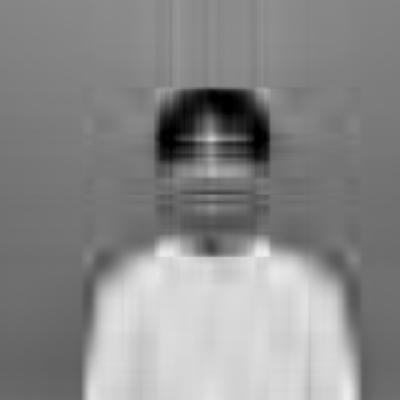
\includegraphics[width=0.2\textwidth]{Q2-2/compressed_k5.jpg} \\
            \hline
            10 & 19.975031210986266 & 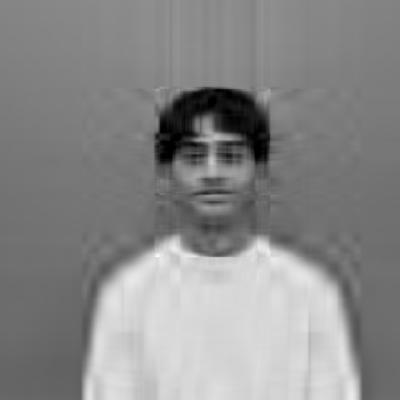
\includegraphics[width=0.2\textwidth]{Q2-2/compressed_k10.jpg} \\
            \hline
            40 & 4.9937578027465666 & 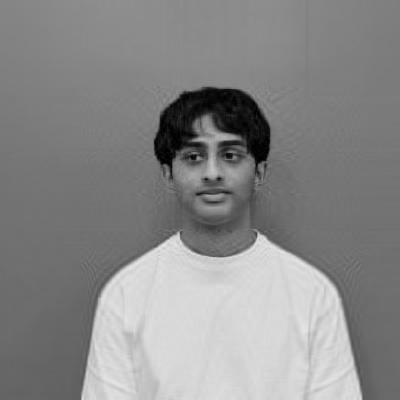
\includegraphics[width=0.2\textwidth]{Q2-2/compressed_k40.jpg} \\
            \hline
            60 & 3.329171868497711 & 
\includegraphics[width=0.2\textwidth]{Q2-2/compressed_k60.jpg} \\
            \hline
        \end{tabular}        
        \caption{Singular Values Retained vs Compression Ratio}
        \label{tab:compression-ratio}
    \end{table}
    \item Original Image vs Compressed Image
        \begin{figure}[H]
            \centering
            \begin{tabular}{cc}
                
\includegraphics[width=0.4\textwidth]{Q2-2/ankkit-art-gallery-grey.jpg} & 
                
\includegraphics[width=0.4\textwidth]{Q2-2/compressed_k60.jpg} \\
                Original Image & Compressed Image (k=60)
            \end{tabular}
            \caption{Original Image vs Compressed Image}
            \label{fig:original-vs-compressed}
        \end{figure}
\end{enumerate}
\end{document}
